% The front cover is in French
\selectlanguage{french}
\newgeometry{inner=30mm,outer=20mm,vmargin=40mm}


%background image of the front cover
\AddToShipoutPicture*{%
    \put(0,0){%
    \parbox[b][42.5cm]{\paperwidth}{%
        \vfill
        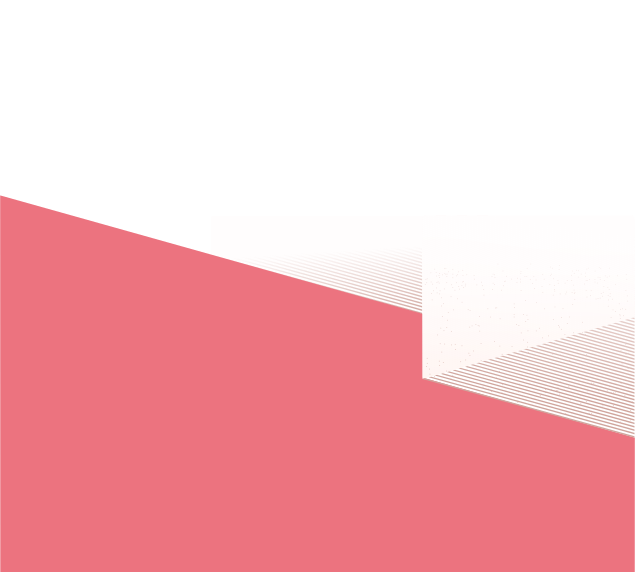
\includegraphics[width=\paperwidth,keepaspectratio]{couverture/image-fond-MATHSTIC-garde.pdf}% image de fond 
        \vfill
}}}




\jury{
\footnotesize %% default for the whole \jury{} block
{\normalsize \textbf{Rapporteurs avant soutenance :}}\par
\vspace{0.25cm}

\begin{tabular}{@{}ll}
Pr{\'e}nom NOM & Fonction et {\'e}tablissement d'exercice \\
Pr{\'e}nom NOM & Fonction et {\'e}tablissement d'exercice \\
Pr{\'e}nom NOM & Fonction et {\'e}tablissement d'exercice \\
\end{tabular}

\vspace{\baselineskip}
{\normalsize \textbf{Composition du Jury :}}\par
{\fontsize{9.5}{11}\selectfont {\textcolor{red}{ %% to remove after defense
\textit{Attention, en cas d’absence d’un des membres du jury le jour de la soutenance, %% to remove after defense
la composition du jury doit être revue pour s’assurer qu’elle est conforme et devra %% to remove after defense
{\^e}tre r{\'e}percut{\'e}e sur la couverture de th{\`e}se}}}}\par  %% to remove after defense
%% remove the line above after the defense, and if jury members could not come, update the following table to remove them
\vspace{0.25cm}

\begin{tabular}{@{}lll}
Pr{\'e}sident :        & Pr{\'e}nom NOM & Fonction et {\'e}tablissement d'exercice \textit{(à préciser après la soutenance)} \\
Examinateurs :         & Pr{\'e}nom NOM & Fonction et {\'e}tablissement d'exercice \\
                       & Pr{\'e}nom NOM & Fonction et {\'e}tablissement d'exercice \\
                       & Pr{\'e}nom NOM & Fonction et {\'e}tablissement d'exercice \\
                       & Pr{\'e}nom NOM & Fonction et {\'e}tablissement d'exercice \\
Dir. de th\`{e}se :    & Pr{\'e}nom NOM & Fonction et {\'e}tablissement d'exercice \\
Encadr. de th\`{e}se : & Pr{\'e}nom NOM & Fonction et {\'e}tablissement d'exercice \\
\end{tabular}

\vspace{\baselineskip}
{\normalsize \textbf{Invit{\'e}(s) :}}\par
\vspace{0.25cm}
%% do not leave blank space with the line above
\begin{tabular}{@{}ll}
Pr{\'e}nom NOM & Fonction et {\'e}tablissement d'exercice \\
\end{tabular}
}


\maketitle

% Restore original margin settings
\restoregeometry
